%==========================================
%
% Latin.Science 2024  template para artigo
% Adaptado de IEEEtran.cls
%
%==========================================
% *** Authors should verify (and, if needed, correct) their LaTeX system  ***
% *** with the testflow diagnostic prior to trusting their LaTeX platform ***
% *** with production work. The IEEE's font choices and paper sizes can   ***
% *** trigger bugs that do not appear when using other class files.       ***                          ***
% The testflow support page is at:
% http://www.michaelshell.org/tex/testflow/

\documentclass[10pt,conference]{IEEEtran}

% Some very useful LaTeX packages include:
% (uncomment the ones you want to load)


% *** MISC UTILITY PACKAGES ***
%
%\usepackage{ifpdf}
% Heiko Oberdiek's ifpdf.sty is very useful if you need conditional
% compilation based on whether the output is pdf or dvi.
% usage:
% \ifpdf
%   % pdf code
% \else
%   % dvi code
% \fi
% The latest version of ifpdf.sty can be obtained from:
% http://www.ctan.org/pkg/ifpdf
% Also, note that IEEEtran.cls V1.7 and later provides a builtin
% \ifCLASSINFOpdf conditional that works the same way.
% When switching from latex to pdflatex and vice-versa, the compiler may
% have to be run twice to clear warning/error messages.

% *** CITATION PACKAGES ***
%
\usepackage{cite}
% cite.sty was written by Donald Arseneau
% V1.6 and later of IEEEtran pre-defines the format of the cite.sty package
% \cite{} output to follow that of the IEEE. Loading the cite package will
% result in citation numbers being automatically sorted and properly
% "compressed/ranged". e.g., [1], [9], [2], [7], [5], [6] without using
% cite.sty will become [1], [2], [5]--[7], [9] using cite.sty. cite.sty's
% \cite will automatically add leading space, if needed. Use cite.sty's
% noadjust option (cite.sty V3.8 and later) if you want to turn this off
% such as if a citation ever needs to be enclosed in parenthesis.
% cite.sty is already installed on most LaTeX systems. Be sure and use
% version 5.0 (2009-03-20) and later if using hyperref.sty.
% The latest version can be obtained at:
% http://www.ctan.org/pkg/cite
% The documentation is contained in the cite.sty file itself.

% *** GRAPHICS RELATED PACKAGES ***
%
\ifCLASSINFOpdf
   \usepackage[pdftex]{graphicx}
  % declare the path(s) where your graphic files are
   \graphicspath{{figs/}}
  % and their extensions so you won't have to specify these with
  % every instance of \includegraphics
   \DeclareGraphicsExtensions{.pdf,.jpeg,.png}
\else
  % or other class option (dvipsone, dvipdf, if not using dvips). graphicx
  % will default to the driver specified in the system graphics.cfg if no
  % driver is specified.
   \usepackage[dvips]{graphicx}
  % declare the path(s) where your graphic files are
   \graphicspath{{../figs/}}
  % and their extensions so you won't have to specify these with
  % every instance of \includegraphics
   \DeclareGraphicsExtensions{.eps}
\fi
% graphicx was written by David Carlisle and Sebastian Rahtz. It is
% required if you want graphics, photos, etc. graphicx.sty is already
% installed on most LaTeX systems. The latest version and documentation
% can be obtained at: 
% http://www.ctan.org/pkg/graphicx
% Another good source of documentation is "Using Imported Graphics in
% LaTeX2e" by Keith Reckdahl which can be found at:
% http://www.ctan.org/pkg/epslatex
%
% latex, and pdflatex in dvi mode, support graphics in encapsulated
% postscript (.eps) format. pdflatex in pdf mode supports graphics
% in .pdf, .jpeg, .png and .mps (metapost) formats. Users should ensure
% that all non-photo figures use a vector format (.eps, .pdf, .mps) and
% not a bitmapped formats (.jpeg, .png). The IEEE frowns on bitmapped formats
% which can result in "jaggedy"/blurry rendering of lines and letters as
% well as large increases in file sizes.
%
% You can find documentation about the pdfTeX application at:
% http://www.tug.org/applications/pdftex

% *** MATH PACKAGES ***
%
\usepackage[cmex10]{amsmath}
% A popular package from the American Mathematical Society that provides
% many useful and powerful commands for dealing with mathematics.
%
% Note that the amsmath package sets \interdisplaylinepenalty to 10000
% thus preventing page breaks from occurring within multiline equations. Use:
\interdisplaylinepenalty=2500
% after loading amsmath to restore such page breaks as IEEEtran.cls normally
% does. amsmath.sty is already installed on most LaTeX systems. The latest
% version and documentation can be obtained at:
% http://www.ctan.org/pkg/amsmath
\usepackage{amsthm}
\newtheorem{definition}{Definition}

% *** SPECIALIZED LIST PACKAGES ***
%
\usepackage{algorithmic}
% algorithmic.sty was written by Peter Williams and Rogerio Brito.
% This package provides an algorithmic environment fo describing algorithms.
% You can use the algorithmic environment in-text or within a figure
% environment to provide for a floating algorithm. Do NOT use the algorithm
% floating environment provided by algorithm.sty (by the same authors) or
% algorithm2e.sty (by Christophe Fiorio) as the IEEE does not use dedicated
% algorithm float types and packages that provide these will not provide
% correct IEEE style captions. The latest version and documentation of
% algorithmic.sty can be obtained at:
% http://www.ctan.org/pkg/algorithms
% Also of interest may be the (relatively newer and more customizable)
% algorithmicx.sty package by Szasz Janos:
% http://www.ctan.org/pkg/algorithmicx

% *** ALIGNMENT PACKAGES ***
%
\usepackage{array}
% Frank Mittelbach's and David Carlisle's array.sty patches and improves
% the standard LaTeX2e array and tabular environments to provide better
% appearance and additional user controls. As the default LaTeX2e table
% generation code is lacking to the point of almost being broken with
% respect to the quality of the end results, all users are strongly
% advised to use an enhanced (at the very least that provided by array.sty)
% set of table tools. array.sty is already installed on most systems. The
% latest version and documentation can be obtained at:
% http://www.ctan.org/pkg/array


% IEEEtran contains the IEEEeqnarray family of commands that can be used to
% generate multiline equations as well as matrices, tables, etc., of high
% quality.

% *** SUBFIGURE PACKAGES ***
\ifCLASSOPTIONcompsoc
  \usepackage[caption=false,font=normalsize,labelfont=sf,textfont=sf]{subfig}
\else
  \usepackage[caption=false,font=footnotesize]{subfig}
\fi
% subfig.sty, written by Steven Douglas Cochran, is the modern replacement
% for subfigure.sty, the latter of which is no longer maintained and is
% incompatible with some LaTeX packages including fixltx2e. However,
% subfig.sty requires and automatically loads Axel Sommerfeldt's caption.sty
% which will override IEEEtran.cls' handling of captions and this will result
% in non-IEEE style figure/table captions. To prevent this problem, be sure
% and invoke subfig.sty's "caption=false" package option (available since
% subfig.sty version 1.3, 2005/06/28) as this is will preserve IEEEtran.cls
% handling of captions.
% Note that the Computer Society format requires a larger sans serif font
% than the serif footnote size font used in traditional IEEE formatting
% and thus the need to invoke different subfig.sty package options depending
% on whether compsoc mode has been enabled.
%
% The latest version and documentation of subfig.sty can be obtained at:
% http://www.ctan.org/pkg/subfig

% *** FLOAT PACKAGES ***
%
%\usepackage{fixltx2e}
% fixltx2e, the successor to the earlier fix2col.sty, was written by
% Frank Mittelbach and David Carlisle. This package corrects a few problems
% in the LaTeX2e kernel, the most notable of which is that in current
% LaTeX2e releases, the ordering of single and double column floats is not
% guaranteed to be preserved. Thus, an unpatched LaTeX2e can allow a
% single column figure to be placed prior to an earlier double column
% figure.
% Be aware that LaTeX2e kernels dated 2015 and later have fixltx2e.sty's
% corrections already built into the system in which case a warning will
% be issued if an attempt is made to load fixltx2e.sty as it is no longer
% needed.
% The latest version and documentation can be found at:
% http://www.ctan.org/pkg/fixltx2e


%\usepackage{stfloats}
% stfloats.sty was written by Sigitas Tolusis. This package gives LaTeX2e
% the ability to do double column floats at the bottom of the page as well
% as the top. (e.g., "\begin{figure*}[!b]" is not normally possible in
% LaTeX2e). It also provides a command:
%\fnbelowfloat
% to enable the placement of footnotes below bottom floats (the standard
% LaTeX2e kernel puts them above bottom floats). This is an invasive package
% which rewrites many portions of the LaTeX2e float routines. It may not work
% with other packages that modify the LaTeX2e float routines. The latest
% version and documentation can be obtained at:
% http://www.ctan.org/pkg/stfloats
% Do not use the stfloats baselinefloat ability as the IEEE does not allow
% \baselineskip to stretch. Authors submitting work to the IEEE should note
% that the IEEE rarely uses double column equations and that authors should try
% to avoid such use. Do not be tempted to use the cuted.sty or midfloat.sty
% packages (also by Sigitas Tolusis) as the IEEE does not format its papers in
% such ways.
% Do not attempt to use stfloats with fixltx2e as they are incompatible.
% Instead, use Morten Hogholm'a dblfloatfix which combines the features
% of both fixltx2e and stfloats:
%
% \usepackage{dblfloatfix}
% The latest version can be found at:
% http://www.ctan.org/pkg/dblfloatfix

% *** PDF, URL AND HYPERLINK PACKAGES ***
%
\usepackage{url}
% url.sty was written by Donald Arseneau. It provides better support for
% handling and breaking URLs. url.sty is already installed on most LaTeX
% systems. The latest version and documentation can be obtained at:
% http://www.ctan.org/pkg/url
% Basically, \url{my_url_here}.




% *** Do not adjust lengths that control margins, column widths, etc. ***
% *** Do not use packages that alter fonts (such as pslatex).         ***
% There should be no need to do such things with IEEEtran.cls V1.6 and later.
% (Unless specifically asked to do so by the journal or conference you plan
% to submit to, of course. )

% correct bad hyphenation here
\hyphenation{op-tical net-works semi-conduc-tor}

% PACOTES RELACIONADOS A ADIÇÃO DO CABEÇALHO DAS PAGINAS
\usepackage[left=1.6cm,top=4cm,right=1.6cm,bottom=1.5cm,headheight=1cm]{geometry}
\usepackage{lipsum}
\usepackage{graphicx}
% utilizado para calcular o tamanho da pagina
\usepackage{tikz}
\usepackage{fancyhdr}
\usepackage{tikzpagenodes}
\usepackage{soulutf8,xcolor}

\renewcommand{\headrulewidth}{0pt}
\renewcommand{\footrulewidth}{0pt}
\renewcommand{\refname}{Referências}
\usetikzlibrary{calc}
\pagestyle{fancy}
\setlength\headheight{10.0pt}
\addtolength{\textheight}{-40.0pt}

\fancyhead[L]{\begin{tikzpicture}[remember picture,overlay]
\draw  let \p1=($(current page.north)-(current page header area.south)$),
      \n1={veclen(\x1,\y1)} in
node [inner sep=0,outer sep=0,below right] 
      at (current page.north west){
\includegraphics[width=\paperwidth,height=\n1]{headerimg.png}};
\end{tikzpicture}}


\fancyfoot[R]{\begin{tikzpicture}[remember picture,overlay]
\draw  let \p1=($(current page footer area.north)-(current page.south)$),
      \n1={veclen(\x1,\y1)} in
node [inner sep=0,outer sep=0,above right] 
      at (current page.south west){
\includegraphics[width=\paperwidth,height=\n1]{footerimg.png}};
\end{tikzpicture}}



 
\begin{document}
%
% paper title
% Titles are generally capitalized except for words such as a, an, and, as,
% at, but, by, for, in, nor, of, on, or, the, to and up, which are usually
% not capitalized unless they are the first or last word of the title.
% Linebreaks \\ can be used within to get better formatting as desired.
% Do not put math or special symbols in the title.

%\title{Exemplo do IEEE adaptado para o Latin.Science 2024}
\title{Avaliação de modelos de implantação de funções serverless no serviço AWS Lambda}
%------------------------------------------------------------------------- 
%------------------------IMPORTANTE---------------------------------------
\newif\iffinal
\finaltrue
%------------------------------------------------------------------------- 
% author names and affiliations
% use a multiple column layout for up to two different
% affiliations
\iffinal
% author names and affiliations
% use a multiple column layout for up to three different
% affiliations
\author{
\IEEEauthorblockN{%1\textsuperscript{st}
Gabriel Duessmann}
\IEEEauthorblockA{\textit{Programa de Pós-Graduação em Computação Aplicada}\\
\textit{Departamento de Ciência da Computação - DCC}\\
\textit{Universidade do Estado de Santa Catarina - UDESC}\\
Joinville, Brasil \\
gabriel.duessmann@edu.udesc.br}
\and
\IEEEauthorblockN{%2\textsuperscript{nd}
Adriano Fiorese}
\IEEEauthorblockA{\textit{Programa de Pós-Graduação em Computação Aplicada}\\
\textit{Departamento de Ciência da Computação - DCC }\\
\textit{Universidade do Estado de Santa Catarina - UDESC}\\
Joinville, Brasil \\
https://orcid.org/0000-0003-1140-0002}
}
% conference papers do not typically use \thanks and this command
% is locked out in conference mode. If really needed, such as for
% the acknowledgment of grants, issue a \IEEEoverridecommandlockouts
% after \documentclass

% for over three affiliations, or if they all won't fit within the width
% of the page, use this alternative format:
% 
%\author{\IEEEauthorblockN{Michael Shell\IEEEauthorrefmark{1},
%Homer Simpson\IEEEauthorrefmark{2},
%James Kirk\IEEEauthorrefmark{3}, 
%Montgomery Scott\IEEEauthorrefmark{3} and
%Eldon Tyrell\IEEEauthorrefmark{4}}
%\IEEEauthorblockA{\IEEEauthorrefmark{1}School of Electrical and Computer Engineering\\
%Georgia Institute of Technology,
%Atlanta, Georgia 30332--0250\\ Email: see http://www.michaelshell.org/contact.html}
%\IEEEauthorblockA{\IEEEauthorrefmark{2}Twentieth Century Fox, Springfield, USA\\
%Email: homer@thesimpsons.com}
%\IEEEauthorblockA{\IEEEauthorrefmark{3}Starfleet Academy, San Francisco, California 96678-2391\\
%Telephone: (800) 555--1212, Fax: (888) 555--1212}
%\IEEEauthorblockA{\IEEEauthorrefmark{4}Tyrell Inc., 123 Replicant Street, Los Angeles, California 90210--4321}}

\else
  \author{ID do artigo Latin.science 2020: \cmtid \\ }
\fi


% make the title area
\maketitle

%utilizado para adicionar header nesta página
\thispagestyle{fancy}


% As a general rule, do not put math, special symbols or citations
% in the abstract

\begin{abstract}
With the advancement of computing and serverless services in the last couple of years, this area is growing. Currently, most cloud providers offer serverless services, in particular at Amazon, they have AWS Lambda to create serverless functions. There are at least two ways to implement a serverless function. One way is to compress the source code and required files in a compacted file in ZIP format, and the other one is through a container image, which has the running application and its dependencies. Depending on the approach chosen, the performance, the cost and the initialization time may vary. Considering these metrics, this paper wants to compare the two approaches mentioned regarding the implementations of serverless functions at AWS and aims to discover whether one of the approaches appears to be the most adequate. Experiments conducted at AWS Lambda show that functions created with compacted ZIP files present advantages, mainly in the initialization time of the function when it is in cold start mode.
\end{abstract}

\renewcommand{\IEEEkeywordsname}{Keywords}
% no keywords
\begin{IEEEkeywords}
Serverless Function, AWS Lambda, Container, Evaluation, Performance, Cost, Start time
\end{IEEEkeywords}

\renewcommand{\abstractname}{Resumo}
%\renewcommand{\abstractname}{Resumen}

\begin{abstract}
 Com o avanço da computação em nuvem e serviços \textit{serverless}, mais foco essa área vem ganhando nos últimos anos. Provedores de nuvem oferecem serviços relacionados a \textit{serverless}, e em particular a Amazon disponibiliza o AWS Lambda para a criação de funções \textit{serverless} pelos seus clientes. Existem ao menos duas forma de implantação de funções \textit{serverless}. Sendo assim, uma forma encapsula o código fonte e demais arquivos necessários em um arquivo compactado no formato ZIP, e outra onde a própria função executável e demais dependências estão em uma imagem de contâiner. Dependendo da abordagem escolhida, o desempenho, o custo e o tempo de inicialização podem variar. Levando em consideração essas métricas, este trabalho visa compará-las entre as duas abordagens de implantação de funções \textit{serverless} e tem como objetivo descobrir se uma das abordagens apresenta ser mais adequada do que outra. Experimentos conduzidos visando tal comparação demonstram que a criação de funções utilizando arquivo compactado ZIP apresentam vantagens, principalmente no tempo de inicialização da função quando está em modo de partida fria.
\end{abstract}

\renewcommand\IEEEkeywordsname{Palavras-chave}

% no keywords
\begin{IEEEkeywords}
Função Serverless, AWS Lambda, Contêiner, Avaliação, Desempenho, Custo, Tempo Inicialização
\end{IEEEkeywords}


% For peerreview papers, this IEEEtran command inserts a page break and
% creates the second title. It will be ignored for other modes.
\IEEEpeerreviewmaketitle



\section{Introdução}
\label{sec:Intro}

\textit{Serverless} é um modelo de computação em nuvem na qual os provedores ofertam serviços de provisionamento dinâmico de servidores configurados para que seus clientes executem suas aplicações. Sendo assim, o provedor \hl{do serviço em nuvem \textit{serverless}} é quem tem a responsabilidade do provisionamento, escalabilidade e segurança das aplicações implantadas nesse modelo \cite{Nupponen_2020_serverless_what_it_is}.
Isso traz maior praticidade para que desenvolvedores e companhias implementem suas aplicações sem a preocupação em contratação e manutenção de infraestrutura necessária para sua execução. 
Cada aplicação implantada nesse modelo, é chamada de função \textit{serverless}, a qual deve executar independentemente da infraestrutura ofertada pelo provedor.

Ao comparar o modelo atual \textit{serverless} com aplicações monolíticas, este possui como principais diferenças: o tamanho e o tempo de execução das aplicações \textit{serverless} são menores, não \st{precisam}\hl{há necessidade} de configurações de um servidor \hl{para executarem} e são automaticamente escaláveis conforme a utilização dos recursos \hl{contratados e} alocados. Já aplicações monolíticas compõem todo o código de um sistema \st{ou grande empresa}, e por isso tendem a terem códigos \hl{fonte} maiores, incluindo longos trechos de código, configurações de servidores e banco de dados. A escalabilidade, além de não ser padrão, pode ser um desafio devido ao grande tamanho da aplicação e necessidade de recursos \st{alocados}\hl{disponíveis para alocação, e muitas vezes ociosos, para atendimento da demanda dos usuários}. Visto que o sistema é executado todo em uma aplicação, para escalar \st{um}\hl{esse tipo de} sistema é preciso que toda a aplicação tenha recursos adicionados. Independente do quão grande ou pequeno o gargalo é no sistema, a aplicação como um todo precisa ser escalada, o que resulta em um desperdício computacional.

Apesar da maior facilidade de desenvolvimento, no sentido da abstração da infraestrutura necessária para a execução e atendimento da demanda elástica da aplicação, a implantação da aplicação no ambiente \textit{serverless} demanda cuidados, pois as configurações do ambiente são feitas pelo provedor e os desenvolvedores não tem acesso para alterá-las. Tais cuidados estão relacionados a \hl{a configuração dos recursos necessários para executá-la, bem como} a forma que a aplicação é instanciada e desativada de acordo com o seu uso \hl{(pelos usuários)} e ociosidade \hl{(períodos sem demanda por parte dos usuários)}. A medida que a aplicação fica ociosa por alguns minutes, o provedor desaloca os recursos computacionais da função, e a mesma fica inoperante. Quando uma nova \st{chamada}\hl{execução} é requisitada à função, e a mesma se encontra nesse estado \hl{inoperante}, o serviço a instancia novamente com os recursos alocados, \hl{o que é chamado} de partida lenta. Quando é feita uma c\st{hamada a}\hl{invocação (por parte do cliente) à} função que se encontra no estado inoperante, o tempo de resposta também é maior na primeira requisição.   

No provedor de nuvem AWS, particularmente, há duas maneiras de se implantar uma nova função manualmente: a maneira mais tradicional via arquivo compactado em \hl{formato} zip, ou através de uma imagem de contêiner, opção introduzida pela empresa em 2020 \cite{aws_2020_supports_container_image}.

Na implantação via arquivo compactado, o desenvolvedor precisa compactar em formato ZIP a pasta do projeto, incluindo o código fonte e os arquivos executáveis da aplicação, e deve realizar o \textit{upload} direto para o serviço \textit{serverless}, \hl{que é chamado AWS Lambda}. Com o uso de imagem de contêiner, é necessário adicionar um arquivo Dockerfile com as dependências e configurações para realizar o \textit{build} da imagem e para executar o projeto. A partir da imagem gerada no ambiente local do desenvolvedor, esta deve ser publicada no repositório de imagens do provedor. \hl{Na sequência,} para se criar então a  função \textit{serverless}, deve ser selecionada a respectiva imagem disponível no repositório. 

Independente do modelo de implantação escolhido, o desenvolvedor precisa implementar no código da aplicação uma interface fornecida pelo serviço AWS Lambda para receber as requisições e parâmetros de entrada \hl{do cliente a utilizará}. Dessa forma, a função \textit{serverless} sabe qual método do código invocar ao receber requisições.

Como contribuição científica, este trabalho busca responder as seguintes perguntas:
\begin{enumerate}
  \item Dentre os modelos de implantação de função \textit{serverless} \st{na Amazo}\hl{no serviço AWS Lambda}, qual é o modelo mais vantajoso, \st{dado as}\hl{de acordo com} métricas de desempenho e tempo de inicialização? 
  \item Como o custo impacta cada uma dessas implantações? 
\end{enumerate}

Para \st{corroborar com as}\hl{subsidiar a} resposta, o trabalho aborda as duas possibilidades de criar/implantar funções \textit{serverless} no serviço AWS Lambda através de experimentos, e propõe uma comparação de desempenho, custo e tempo de inicialização entre as abordagens. Por fim, busca-se \st{concluir}\hl{avaliar} se há um modelo de implantação mais vantajoso do que outro.

Para \st{chegar nos}\hl{obter os} resultados de comparação,\st{testes foram}\hl{experimentos são} executados nas funções \textit{serverless} via chamada de API. As métricas \st{analisadas foram}\hl{de desempenho para realizar tal comparação são as} de consumo máximo de memória, o custo para implantar as funções e o tempo de inicialização da \hl{função/}aplicação. Durante a execução \st{de testes}\hl{dos experimentos}, é utilizado o acesso \textit{Free Tier} \hl{ao serviço AWS Lambda}, e não houve cobrança nos serviços utilizados. Portanto, a comparação de custo se deu com base nos valores estimados que são informados pela empresa Amazon.

Esse artigo é estruturado da seguinte maneira: A Seção \ref{sec:RefTeo} apresenta o referencial teórico para esclarecer termos relacionados a nuvem e ao provedor AWS, \hl{incluindo o serviço AWS Lambda}, \hl{bem como}\st{e} apresenta\st{r} características utilizadas na avaliação. A Seção \ref{sec:TrabRel} \st{lista}\hl{elenca} trabalhos relacionados pertinentes ao tema, bem como suas características e como se diferem desse artigo. Na Seção \ref{sec:experiments}, é apresentada a proposta de avaliação \hl{de implantação de aplicações \textit{serverless}}, bem como os experimentos realizados e \hl{os valores d}as métricas coletadas. Por fim, a Seção \ref{sec:Conclusion} conclui o artigo.

\section{Referencial Teórico} 
\label{sec:RefTeo}

Com o avanço da computação em nuvem, cada vez mais serviços estão sendo migrados ou implementados nesse modelo. Os provedores de nuvem, por sua vez, estão dedicados a criarem e disponibilizarem recursos que melhoram a qualidade e praticidade de seus serviços a fim de atender um maior número de clientes. Um desses serviços é o chamado \textit{serverless}, que executa uma aplicação sem que o cliente necessite configurar o servidor e demais infraestruturas. \hl{Nesse sentido, esta seção trata de temas pertinentes a avaliação proposta passando pelo modelo de computação em nuvem; definindo funções \textit{serverless}; os modelos de implantação \textit{serverless}, no serviço AWS Lambda em particular, incluindo a conceituação de \textit{containers}; e os serviços da nuvem computacional AWS da empresa Amazon, incluindo o AWS Lambda e correlacionados à disponibilização do serviço \textit{serverless}}. %o uso de \hl{No  serviço \textit{serverless}, geralmente,} \st{A implantação de} uma aplicação \st{em \textit{serverless}} é chamada de função \textit{serverless}. Para que a aplicação seja executada como um função, o desenvolvedor precisa adicionar em seu código as dependências disponibilizadas pelo provedor. Em específico, a implementação necessária para a AWS é abordada na Seção \ref{subsec:aws_services}.
    
\subsection{Computação em Nuvem}
\label{subsec:cloud}

A computação em nuvem é um modelo \hl{de disponibilização de serviços computacionais} \st{com vastos recursos de computação} compartilhados, como rede, servidores, armazenamento, aplicações e serviços que podem ser provisionados e liberados \hl{sob demanda} rapidamente e com baixa configuração e complexidade \hl{por parte dos seus usuários} \cite{nist_2011_cloud_computing}.
Os provedores de nuvem são responsáveis por cuidar, controlar e ofertar serviços em nuvem para usuários finais ou entidades \hl{que necessitam de poder computacional, mas que não querem ter o custo de propriedade e operação dos equipamentos físicos envolvidos}. Conforme os clientes utilizam os serviços ofertados, pagam sob demanda de acordo com a utilização dos mesmos ou conforme acordo firmado com o provedor. Com a computação em nuvem, \textit{data centers} e infraestruturas de empresas começaram a ser migrados para nuvem devido a agilidade e praticidade dos serviços ofertados pelos provedores. Como consequência, as aplicações também precisaram ser migradas, o que leva a novas formas de aproveitamento dos recursos computacionais disponíveis, tendo em vista a otimização dos mesmos e do custo, dado o modelo de precificação baseado no pagamento do que é usado sob demanda.

\subsection{Função serverless}
\label{subsec:serverless_funcion}

\hl{O modelo de computação}\st{Funções} \textit{serverless} \hl{é um modelo de serviço de computação em nuvem, também conhecido por funções \textit{serverless}} ou modelo \textit{Function as a Service} (FaaS) \hl{que} providencia a abstração dos servidores e demais infraestrutura\hl{, para a execução de aplicações em nuvem, sob demanda, sem necessidade de alocação (uso de recursos computacionais) prévia}. Assim, os clientes do modelo, ou seja, os desenvolvedores de aplicações, precisam apenas implementar o código da aplicação, isto é, a função. Ao ter \hl{em suas instalações} o código implementado \hl{da aplicação}, o provedor toma conta de \hl{alocar/}instanciar o servidor físico ou virtual, configurar o ambiente e disponibilizar uma \textit{Application Program Interface} (API) para acesso da aplicação por parte do \st{cliente}\hl{usuário final} da mesma. 

Uma das principais vantagens desse modelo é que o provedor \hl{de serviço \textit{serverless}} é responsável pela escalabilidade da aplicação. A escalabilidade nesse caso contempla a instanciação da função para sua utilização pelos \st{clientes}\hl{usuários finais} da aplicação, de forma a atender a demanda de requisições, bem como o gerenciamento dessas instâncias quando não estão necessariamente atendendo às requisições dos clientes finais. É possível utilizar estratégias de otimização com vistas a reutilização dos recursos para o atendimento da escalabilidade.
Uma das estratégias utilizadas para gerenciar o \st{dimensionamento}\hl{a alocação} dos recursos\hl{tendo em vista a escalabilidade} é chamada de \textit{cold start}, ou partida lenta. 
\hl{Nesse caso,} conforme a função deixa de ser utilizada \hl{pelos usuários finais}, os recursos de \textit{hardware} alocados passam a ficar ociosos, e portanto, os provedores desalocam parte desses recursos para obter uma maior economia em seus servidores \hl{possibilitando o uso desses recursos em outras funções \textit{serverless} ou sistemas}. Quando a aplicação é novamente invocada \hl{por um usuário final}, \hl{ela} pode necessitar que os recursos sejam reativados e uma nova instância seja criada. Esse processo é chamado de partida lenta ou fria \cite{vahidinia_2020_cold_start}. Após ter os recursos reativados, essa instância permanecerá ativa enquanto é utilizada, e por um período de tempo (minutos) após a sua \hl{última} utilização\hl{, ou seja, mesmo não sendo utilizada por usuários finais}. \hl{Nesse caso, se nesse período de tempo houver um novo acesso a função por usuários finais, a função \textit{serverless} continua ativa, com os recursos computacionais ativos e alocados a ela. Assim, ela pode ser utilizada de imediato,} processo que é chamado de partida quente, pois \hl{o provedor de serviço \textit{serverless}} possui a instância e os recursos operantes \cite{Raje_2023_cold_warm_start} para o atendimento de nova requisição, \hl{ou seja, continuam ativos ("quentes"),} sem que se\hl{ja necessária} \st{instancie} uma nova instância da função. A função, após ficar alguns minutos ociosa, sem nenhuma execução, tem seus recursos desativados pelo provedor. Esse ciclo continua alternando entre partida fria e partida quente conforme a sua utilização.

O tempo de partida lenta é normalmente considerado uma desvantagem, e otimizações para diminuí-lo são estudados em busca de evitar grandes atrasos ao cliente final. Porém, há dificuldades em se alcançar soluções ideais, dado que as configurações acerca do gerenciamento dos recursos e das instanciações são mantidas pelos provedores de nuvem \cite{vahidinia_2020_cold_start, kumari_2022_mitigating_cold_start, vahidinia_2023_mitigating_cold_start, dantas_2022_reducing_cold_start}, e não são disponíveis para experimentações e otimizações\hl{, por parte dos clientes desses provedores de serviço}.

\subsection{Contêineres}
\label{subsec:containers}

Contêineres fornecem às aplicações um ambiente \hl{computacional para a execução de aplicações, }configurado com todas as suas dependências para ser executado. Eles isolam a aplicação de programas e processos externos que executam no sistema operacional hospedeiro \hl{do contêiner}. Portanto, pode ser definido como um mecanismo de empacotamento de aplicações \cite{Siddiqui_2019_analysis_container}. 

A utilização de contêineres se tornou amplamente popular pela facilidade de migrar aplicações de um ambiente para outro sem a ocorrência de problemas \st{ao}\hl{ocasionados pela} execu\st{tar}\hl{ção} em máquinas diferentes. Sem isso, toda vez que as aplicações migravam para um novo ambiente, havia uma grande chance de ocorrerem erros, pois dois ambientes nunca são totalmente idênticos em questão de \textit{software} e \textit{hardware}, e portanto, podem não ter as configurações e dependências necessárias para a execução da aplicação  \cite{Siddiqui_2019_analysis_container}. Sem o uso de contêineres ou alguma técnica de virtualização, ou seja, em \textit{bare metal}, para cada vez que a aplicação executasse em uma máquina diferente, seria necessário antes disso, instalar suas dependências, programas de terceiros, configurar o ambiente, entre outros.

Para que uma aplicação seja portável entre máquinas com contêiner \hl{é necessário que o \textit{host} hospedeiro, em seu sistema operacional, esteja preparado para a execução de contêineres. Geralmente, alguma instalação e configuração de um software gerenciador de contêineres é necessária. Em um ambiente de nuvem computacional, a depender do modelo de serviço (ex: \textit{Infrastructure as a Service} (IaaS), \textit{Software as a Service} (SaaS), ou mesmo \textit{Function as a Service} (FaaS)) é necessário que o cliente faça tal instalação, ou a mesma é disponibilizada como parte do serviço pelo provedor de nuvem. Além disso,}é preciso de uma imagem \hl{computacional} da aplicação com tudo o que é necessário para executá-la. Com a imagem criada, o contêiner pode ser replicado para outras máquinas de diferentes \textit{hardwares} e sistemas operacionais (SOs) \hl{(e eventualmente diferentes provedores de nuvem)}, mantendo o mesmo funcionamento da aplicação. Isso é possível porque os contêineres são uma forma de virtualização leve, que pode incluir seu próprio SO \cite{scheepers_2014_virtualization_containerization}. Sendo assim, pode-se ter uma imagem de contêiner para cada função \textit{serverless} que se deseja criar e especificar qual imagem utilizar ao criar uma nova função no \hl{serviço} AWS Lambda. 


\subsection{Serviços AWS}
\label{subsec:aws_services}

Um dos maiores provedores de nuvem da atualidade é a AWS (Amazon Web Service), que oferta centenas de serviços disponíveis na Internet. Dentre os serviços ofertados, este trabalho utiliza três deles: AWS Lambda, API Gateway e AWS \textit{Elastic Container Registry} (ECR).

O serviço de \textit{serverless} da Amazon é chamado de AWS Lambda, e nele, consegue-se criar funções para executar aplicações sem precisar provisionar e gerenciar servidores. 
O serviço Lambda gerencia toda a configuração computacional, que oferece equilíbrio de memória, CPU, rede e outros recursos necessários para executar o código da aplicação (função).
As funções são instanciadas sob demanda conforme requisições feitas por usuários finais, o que faz o serviço alocar parte da máquina virtual para a função. Conforme a função passa a ficar ociosa por alguns minutos, os recursos computacionais alocados são desativados. Isso possibilita que os clientes paguem apenas pelo tempo em que a aplicação está sendo utilizada, com os recursos alocados para a função \textit{serverless} \cite{aws_2023_what_is_lambda}.

Para implantar uma aplicação em função \textit{serverless}, é necessário que o desenvolvedor importe em seu projeto as bibliotecas da AWS Lambda específicas para cada linguagem de programação e implemente a interface do serviço \textit{serverless} disponibilizada pela biblioteca específica. Ao criar a função, na etapa de configuração, é necessário informar o caminho do método que implementa a interface, pois esse método é usado como ponto de entrada para a função invocar a aplicação e passar os parâmetros de entrada.

Particularmente, na AWS, há duas maneiras de implantar uma função \textit{serverless}, que são: via arquivo compactado do código fonte ou com uma imagem de contêiner. Para a abordagem de arquivo compactado, é necessário compilar os arquivos fontes, compactar a pasta do projeto em formato ZIP e fazer o \textit{upload} diretamente no serviço AWS Lambda. Com o uso de uma imagem de contêiner, é necessário que o desenvolvedor tenha a imagem publicada na AWS ECR, que é o repositório de imagens de contêineres, e selecionar a respectiva imagem quando da criação da função.

Além das características citadas acerca do servico AWS Lambda, e seus coadjuvantes relacionados ao modelo \textit{serverless}, a arquitetura de \textit{hardware} onde é executada a função também pode ser escolhida junto ao provedor AWS. Assim, ao criar uma nova função, esta pode ser criada sob arquitetura arm64 ou x86\_64. Apesar da arquitetura x86\_64 ser a padrão, a arquitetura arm64 se destaca por possuir menor custo de execução e atingir \st{melhores}\hl{bons} resultados de desempenho
\cite{aws_2023_aws_lambda_architectures}.

AWS ECR é um serviço de repositório para armazenar imagens de contêineres. \hl{Em particular o formato de contêiner utilizado é o formato \textit{docker}.} O desenvolvedor deve criar a imagem em sua máquina local a partir de um arquivo Dockerfile e publicá-la no repositório \cite{aws_2023_aws_ecr}. Assim, ao ter a imagem disponível no repositório, esta pode ser usada em outros serviços do provedor, como por exemplo para criar funções \textit{serverless}.

Amazon API Gateway é um serviço para criar, publicar e gerenciar \st{APIs}\hl{aplicações web??}, \st{podendo ser}\hl{aceitando o formato} REST, HTTP ou WebSocket. É usado como um ponto de entrada para os serviços AWS, incluindo o AWS Lambda, e as APIs podem ser criadas para acessarem os serviços criados ou dados armazenados. Esse serviço lida com as tarefas de aceitar e processar as requisições, com capacidade de processar centenas de milhares de requisições concorrentes \cite{aws_2023_what_is_api_gateway}. \ul{acho que poderias dizer que é por meio desse serviço, ou seja, geralmente por meio da URL HTTP disponibilizada por esse serviço que a função é invocada pelo usuário final, e que dá início ao processo de instanciação da mesma via partida fria ou quente}


\section{Trabalhos Relacionados}
\label{sec:TrabRel}

Modelos FaaS não são tão recentes, e apesar de trazerem praticidade para implementação de aplicações, há ainda espaço para estudos analisarem pontos de melhoria.

O trabalho \cite{dantas_2022_reducing_cold_start} aborda estratégias para diminuir o \textit{cold start} e compara o impacto no tempo ao instanciar uma função através de arquivo compactado e via imagem de contêiner. Apesar de propor soluções para minimizar o tempo de inicialização, o trabalho citado não aborda custo.

Em \cite{Elsakhawy_2021_performance_analysis_serverless}, são investigados os fatores que afetam o desempenho de funções \textit{serverless} e como também são examinados os resultados em opções de contêineres, diferentes linguagens de programação e alternativas de compilações. Porém, os autores do trabalho citado não levam em consideração o custo para executar a função e tempo de inicialização do \textit{cold start}.

Na publicação \cite{Villamizar_2017_cost_comparison_lambda}, os autores compararam os custos de executar aplicações em monolito, microserviço e função Lambda na AWS. Das três arquiteturas, AWS Lambda obteve o menor custo, reduzindo os custos de infraestrutura em 70\%.

Apesar de trabalhos anteriores já terem comparado os modelos de implantação entre arquivo compactado e imagem de contêiner, o trabalho atual busca relacionar suas diferenças considerandos os fatores de desempenho, custo e tempo de inicialização.

A Tabela \ref{tab:related_papers} compara características de alguns trabalhos relacionados e pontua como esse artigo se difere dos demais. As colunas de arquivo compactado e imagem de contêiner são referentes ao modo de implantação da aplicação. As demais colunas apresentam desempenho, custo e tempo de inicialização como métricas referentes às funções.

\begin{table*}[htb]
    \centering
    \caption{Comparação de trabalhos relacionados}
    \label{tab:related_papers}
    \begin{tabular}{ccccccc}
        \hline
         Artigo & Arquivo compactado & Imagem de contêiner & Desempenho & Custo & Tempo de inicialização \\
        \hline
         Dantas\cite{dantas_2022_reducing_cold_start} & Sim & Sim & Não & Sim & Sim \\
        \hline
         Elsakhawy\cite{Elsakhawy_2021_performance_analysis_serverless} & Não  & Sim & Sim & Sim & Não \\
        \hline
         Villamizar\cite{Villamizar_2017_cost_comparison_lambda} & Não & Não & Não & Sim & Não \\
        \hline
         Trabalho atual & Sim & Sim & Sim & Sim & Sim \\
        \hline
    \end{tabular}   
\end{table*}

\section{Metodologia e Experimentos}
\label{sec:experiments}

Este trabalho propõe avaliar dois métodos de implantação de uma aplicação no serviço \textit{serverless} da Amazon, AWS Lambda.
A escolha da linguagem de programação para a aplicação (função) foi Java, devido a sua popularidade no meio Web e facilidade de implementar as interfaces requeridas para o serviço na AWS.

Os experimentos buscam auxiliar na descoberta se uma das abordagens é mais vantajosa que a outra. Para chegar em tal conclusão, métricas pertinentes ao serviço foram analisadas. As métricas levadas em consideração foram de desempenho com base no consumo de memória, de custo e de tempo de inicialização em partida lenta. 

Para realizar a comparação das métricas, foi desenvolvido uma aplicação, implantada como função \textit{serverless} no \hl{serviço} AWS Lambda via \hl{código da função compactado como} arquivo ZIP e imagem de contêiner, e fazendo requisições HTTP via Amazon Gateway.

\st{Primeiro}\hl{Inicialmente}, é descrito o ambiente e as configurações utilizadas, e em seguida, são apresentados as métricas selecionadas e os dados da comparação entre os modelos de implantação.


\subsection{Ambiente}
\label{subsec:environment}

Para realizar tal avaliação, foi realizada a implementação de uma aplicação simples utilizando a linguagem de programção Java, versão 11. A aplicação pode ser considerada simples, pois possui apenas umas interface de entrada de dados onde deve ser informada uma região \hl{geográfica do globo terrestre} e é retornado a data e o horário da região informada. 

Para implantar a aplicação no serviço da AWS, foi criada uma função utilizando arquivo ZIP compactado e outra função via imagem de contêiner. Para criar a função com o uso da imagem, uma imagem da aplicação foi criada a partir de um \hl{arquivo de configuração} Dockerfile \hl{para o formato de contêiner docker,} configurado para realizar o \textit{build} \hl{(instalação do sistema operacional, dependências e a própria aplicação em uma imagem executável, no contêiner)} e publicada no repositória do AWS ECR. \st{Refente a}\hl{A} arquitetura escolhida para as funções foi \st{escolhido} a arquitetura arm64 devido ao menor \st{preço}\hl{custo, bem como a pouca necessidade de processamento, armazenamento ou memória da função (o que se reflete inclusive no custo)}.

Para fazer requisições às funções criadas, optou-se por usar APIs públicas REST na Amazon API Gateway, as quais foram configuradas para invocar as respectivas funções, dependendo do caminho do \textit{endpoint}. É importante utilizar caminhos diferentes para as APIs, pois essas desconhecem o modelo de implantação de cada função \textit{serverless} invocada.

O ambiente configurado é representado no diagrama da Figura \ref{fig:env_diagram}. \hl{Nele,} inicialmente, o usuário faz uma chamada de requisição REST. A requisição é recebida pela API Gateway, que possui um gatilho e redireciona para a respectiva função \textit{serverless} criada. A função pode executar a aplicação implantada via arquivo compactado ZIP ou com uma imagem de contêiner armazenada no Amazon ECR. Ao executar o trecho de código da aplicação, a função \textit{serverless} providencia uma mensagem de resposta para o serviço de API Gateway, o qual redireciona a mensagem para o usuário. \ul{quantas execuções da mesma função foram realizadas? acho importante destacar todos os aspectos dos experimentos aqui.}

\begin{figure}[htbp]
    \centering 
    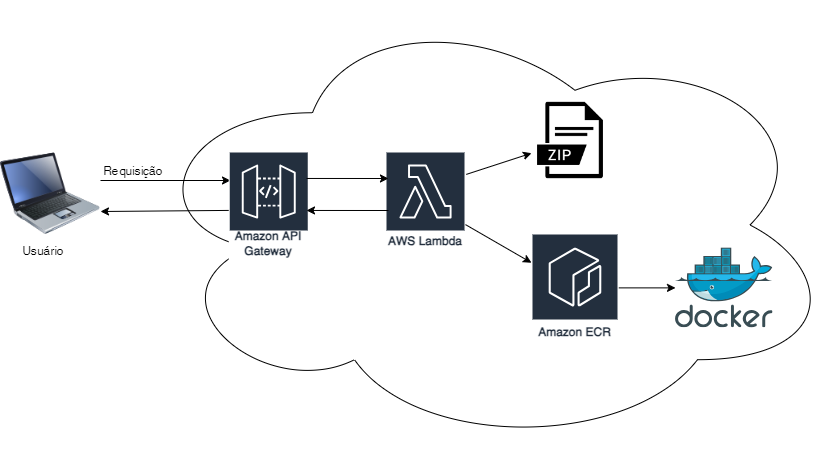
\includegraphics [width=\linewidth]{images/environment-diagram-PT.png}
    \par
    \caption{Diagrama do ambiente de testes}
    \label{fig:env_diagram}
\end{figure}

\subsection{Custo}
\label{subsec:cost}

Para a execução dos experimentos na AWS, não houve incidência de cobrança do provedor por terem sido utilizados apenas serviços e configurações dentro do nível \textit{Free Tier}. Esse nível possibilita que clientes utilizem serviços de forma gratuita, desde que atendam as restrições existentes. Portanto, para comparar o custo entre as duas abordagens de implantação, são usados os valores base de precificação do provedor de nuvem AWS.

O custo para implantar e manter a função \textit{serverless} ativa é o mesmo, independente da abordagem escolhida. Outros fatores, como configuração de \textit{hardware} e localização do servidor podem impactar no valor final, mas estão fora do escopo deste trabalho.
Ao fazer o \textit{upload} do projeto compactado com tamanho até 10 Mb, não há nenhuma cobrança para armazenar os arquivos. Porém, para projetos maiores, é necessário armazená-los no \hl{serviço} S3\hl{, que é o serviço de armazenamento de dados de grande porte do provedor AWS}. Para disponibilizar uma imagem de contêiner no serviço AWS ECR, há um custo, que é proporcional ao tamanho da imagem. A precificação na AWS ECR também varia dependendo da região \cite{aws_2023_ecr_pricing} \hl{de localização do \textit{data center}}. \ul{em que região armazenaste a tua função. Acho que é importante comentar isso para reproducibilidade.}

\subsection{Desempenho}
\label{subsec:performance}

\st{Algumas}\hl{Várias} métricas podem estar relacionadas ao desempenho de uma aplicação. Neste trabalho, \hl{em relação ao desempenho} foi analisado o consumo de memória RAM máximo no ambiente \hl{experimentado} ao executar funções \textit{serverless} que estavam em modo de partida lenta. Essa métrica é coletada no console de saída do AWS Lambda ao fazer uma requisição.

Conforme a Figura \ref{graph:functions_max_memory_used}, nota-se que o uso de memória máximo com a abordagem de imagem de contêiner se mantém constante, enquanto via arquivo ZIP, há uma variação de uma execução para outra. A Figura \ref{graph:functions_max_memory_used_average} apresenta a média de ambas abordagens, corroborando os resultados da Figura \ref{graph:functions_max_memory_used}, demonstrando que a implantação da função feita a partir da imagem de contêiner obteve melhores resultados em relação ao consumo de memória, ou seja, consome menos memória para executar a função. 

\begin{figure}[htbp]
    \centering 
    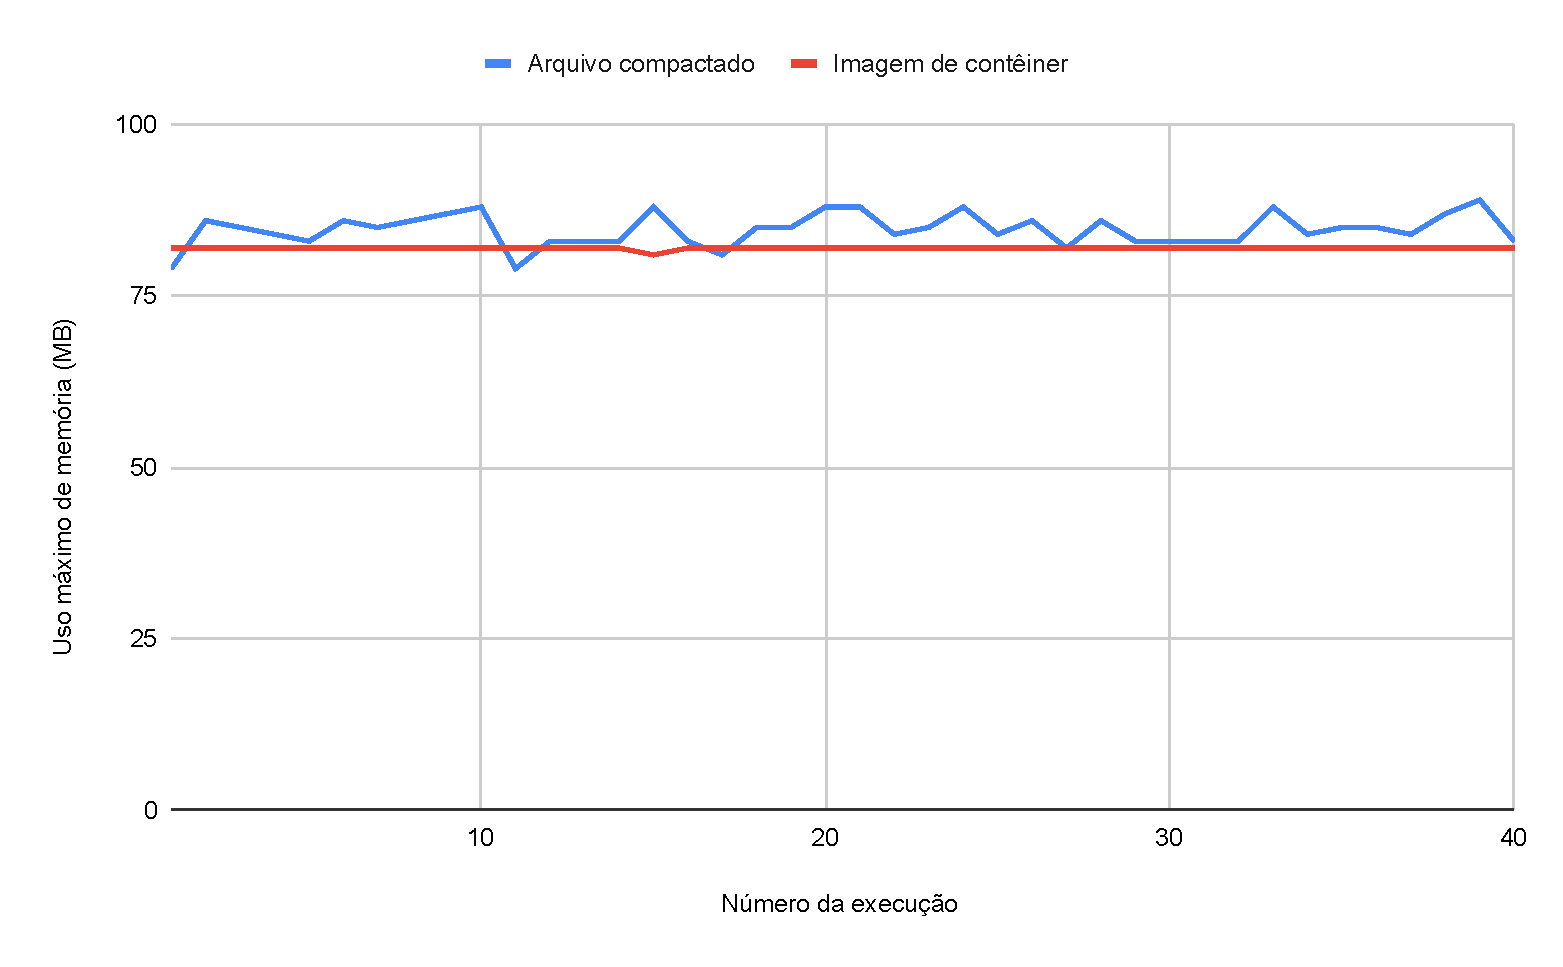
\includegraphics [width=\linewidth]{images/max-memory-use-PT.pdf}
    \par
    \caption{Gráfico de uso de memória máximo em funções \textit{serverless}}
    \label{graph:functions_max_memory_used}
\end{figure}

\begin{figure}[htbp]
    \centering 
    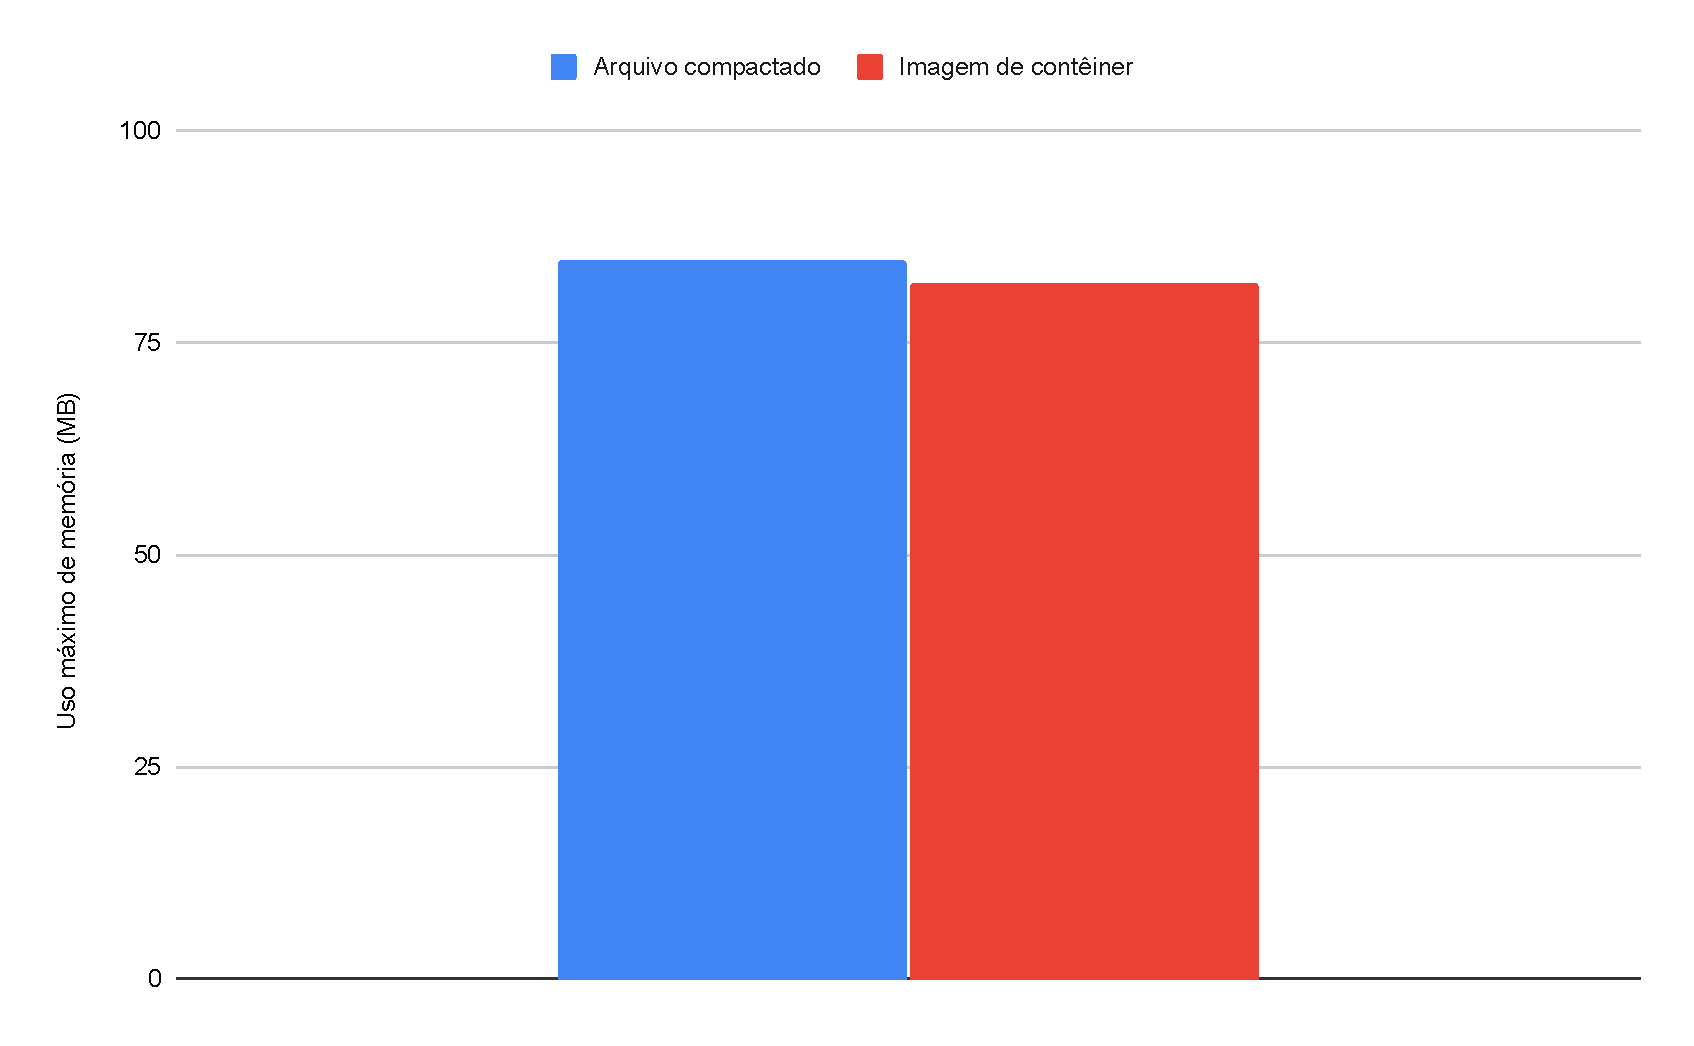
\includegraphics [width=\linewidth]{images/max-memory-use-average-PT.pdf}
    \par
    \caption{Gráfico da média de uso de memória máximo em funções \textit{serverless}}
    \label{graph:functions_max_memory_used_average}
\end{figure}

\subsection{Tempo de inicialização em partida fria} 
\label{subsec:cold_start_time}

As Figuras \ref{graph:functions_init_time} e \ref{graph:functions_init_time_average} \st{mostram}\hl{ilustram} que o método de implantação via arquivo ZIP possui o menor tempo de inicialização \hl{em partida fria???}. Particularmente, observa-se na Figura \ref{graph:functions_init_time} o tempo de inicialização da função implantada via arquivo compactado e via contêiner, para várias inicializações. Cada inicialização ocorreu respeitando tempo suficiente para que os recursos fossem desalocados, obrigando uma nova instanciação da função. A Figura \ref{graph:functions_init_time_average} apresenta a média dos tempos de inicialização apresentados na Figura \ref{graph:functions_init_time}.

O tempo de inicialização também impacta no tempo de resposta quando a aplicação está em modo de partida lenta, portanto, funções executando com arquivo compactado obtém melhores resultados \hl{quanto a inicialização em partida fria}. \ul{não testaste em partida quente? E a comparação entre as métricas, já que em contêiner tem um consumo de memória constante e melhor naquele sentido, segundo o que escreveste. Como fica a conclusão final?}

\begin{figure}[htbp]
    \centering 
    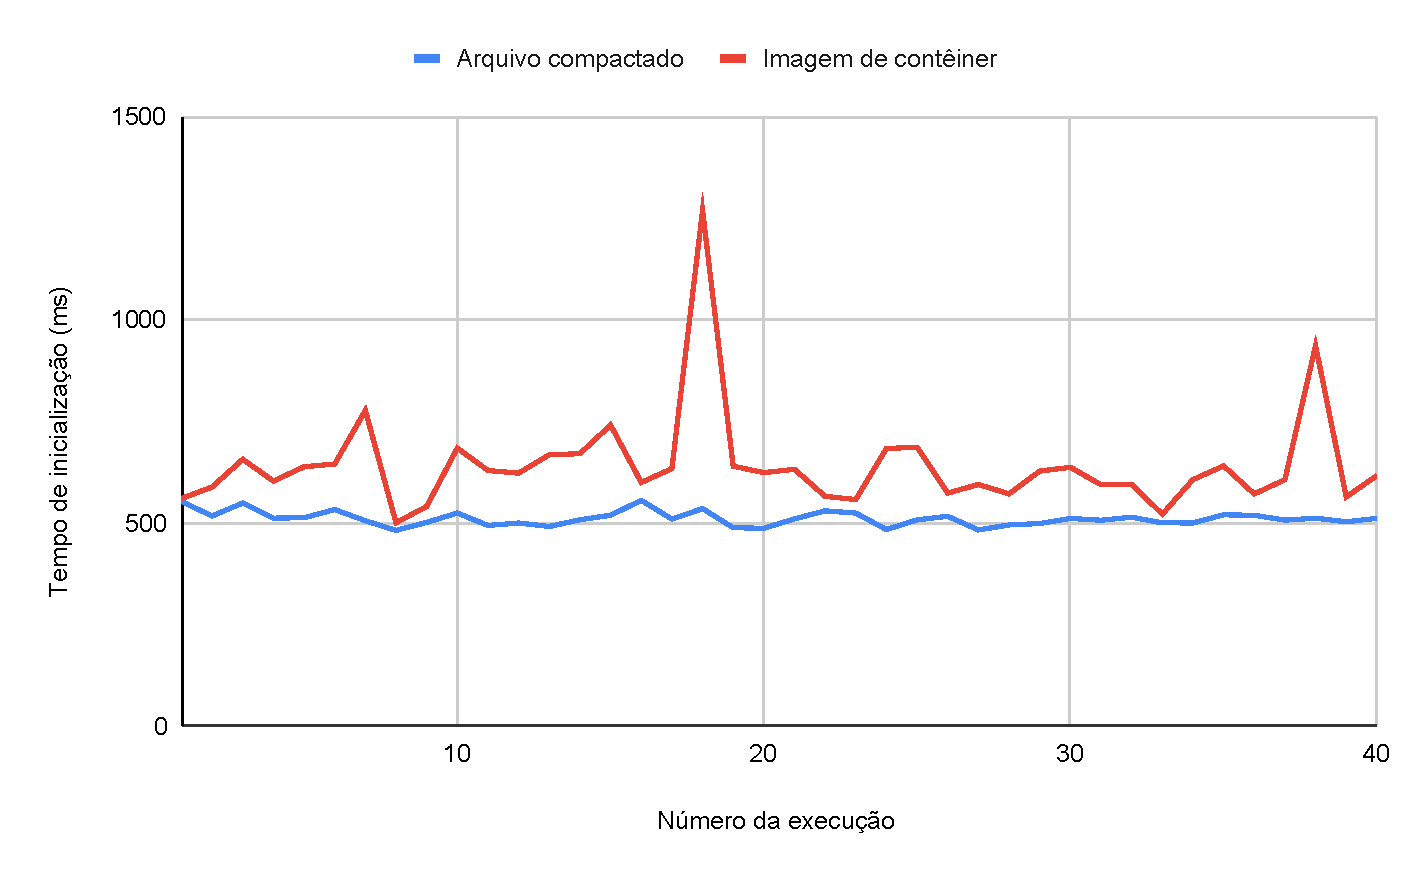
\includegraphics [width=\linewidth]{images/init-time-PT.pdf}
    \par
    \caption{Gráfico do tempo de inicialização em funções \textit{serverless}}
    \label{graph:functions_init_time}
\end{figure}

\begin{figure}[htbp]
    \centering 
    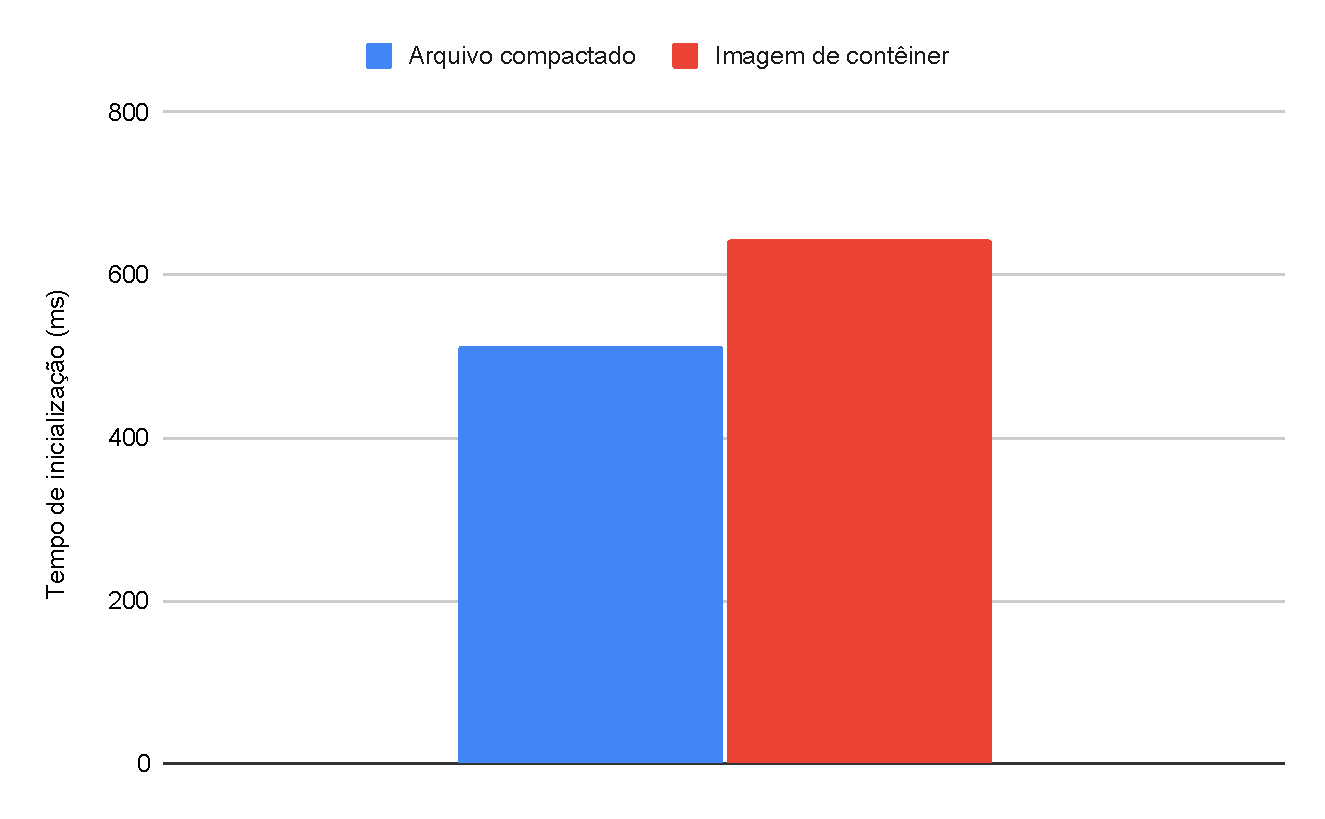
\includegraphics [width=\linewidth]{images/init-time-average-PT.pdf}
    \par
    \caption{Gráfico da média do tempo de inicialização em funções \textit{serverless}}
    \label{graph:functions_init_time_average}
\end{figure}

\section{\st{Conclusão}\hl{Considerações Finais}}
\label{sec:Conclusion}

Esse trabalho avaliou os modelos de implantação de funções \textit{serverless} disponíveis no serviço AWS Lambda. O serviço oferece duas possibilidades \hl{de implantação de funções}: via arquivo compactado no formato ZIP e via imagem de contêiner. Com os arquivos compactados ZIP, o modelo de implantação é mais \st{fácil}\hl{simplificado}, pois \st{é necessário apenas fazer-se}\hl{basta efetuar} o \textit{upload} do projeto \hl{(código da função compactado)} para o serviço AWS Lambda, enquanto que na segunda abordagem é necessário configurar um arquivo Dockerfile para \st{fazer}\hl{executar} o \textit{build} da aplicação, gerar uma imagem de contêiner e publicá-la na AWS ECR.

Como resposta as perguntas estabelecidas \st{no Capítulo}\hl{na Seção} \ref{sec:Intro}, conclui-se que dependendo do modelo escolhido, o custo, o desempenho e o tempo de inicialização da partida lenta podem ser diferentes.
Ao criar as funções \textit{serverless} na AWS Lambda nos dois modelos de implantação, ambos não tiverem incidências de custos durante os testes realizados. Porém, quando a abordagem escolhida é com o uso de uma imagem de contêiner, é necessário utilizar outro serviço para armazenar a imagem, nesse caso o AWS ECR, e este pode vir a gerar custos conforme o tamanho da imagem. Ao analisar o uso máximo de memória RAM quando a aplicação está em modo de partida lenta, ambos apresentaram consumo similar, com a vantagem que via imagem de contêiner o uso da memória se manteve constante. A maior diferença se deu no tempo de inicialização da aplicação em partida lenta, no qual a implantação via arquivo ZIP mostrou-se mais eficiente para alocar os recursos e tornar a função ativa novamente.

Portanto, com base \hl{no cenário experimentado,} nos dados e resultados obtidos e em sua análise, \st{é} pode-se\st{r} inferir que a implantação via arquivo ZIP apresenta vantagens. As principais vantagens comparadas ao modelo de implantação com imagem de contêiner são: o custo para implantação, uma vez que não é necessário armazenar a pasta compacta em outro serviço e o tempo de inicialização quando em partida lenta que é menor.  

Como trabalho futuros, pode-se estender a comparação para as outras linguagens de programação suportadas pelo provedor de nuvem \hl{computacionail} AWS. Outro aspecto a ser comparado é a arquitetura na qual a função \textit{serverless} é executada, x86\_64 ou arm64. Neste trabalho, foi utilizado apenas a arquitetura arm64, havendo espaço para tratar da arquitetura x86\_64. O escopo da aplicação também pode ser extrapolado para aplicações maiores ou mais complexas que demandem maior processamento computacional, e que \st{deve}\hl{presumivelmente podem} impactar no consumo máximo de memória e tempo de inicialização. \st{Aplicações maiores que 10 MB podem ter incidência de custos para disponibilizar o arquivo compactado, o que tornaria a comparação de custo mais justa.}\hl{Ainda, o tamanho da aplicação é outra característica que pode ser explorada em trabalhos futuros, uma vez que a incidência de custo financeiro é diretamente ligada a ela.}

% An example of a double column floating figure using two subfigures.
% (The subfig.sty package must be loaded for this to work.)
% The subfigure \label commands are set within each subfloat command,
% and the \label for the overall figure must come after \caption.
% \hfil is used as a separator to get equal spacing.
% Watch out that the combined width of all the subfigures on a 
% line do not exceed the text width or a line break will occur.
%
%\begin{figure*}[!t]
%\centering
%\subfloat[caso 1]{\includegraphics[width=2.5in]{figs/logo_grupo.png}%
%\label{fig_first_case}}
%\hfil
%\subfloat[caso 2]{\includegraphics[width=2.5in]{figs/logo_grupo.png}%
%\label{fig_second_case}}
%\caption{Latinoware - Congresso Latino-americano de Software Livre e Tecnologias Abertas.}
%\label{fig_sim2}
%\end{figure*}
%
% Note that often IEEE papers with subfigures do not employ subfigure
% captions (using the optional argument to \subfloat[]), but instead will
% reference/describe all of them (a), (b), etc., within the main caption.
% Be aware that for subfig.sty to generate the (a), (b), etc., subfigure
% labels, the optional argument to \subfloat must be present. If a
% subcaption is not desired, just leave its contents blank,
% e.g., \subfloat[].


% use section* for acknowledgment
\section*{Agradecimentos}

Coloque aqui seus agradecimentos.

\bibliographystyle{IEEEtran}
\bibliography{IEEEexample}


\end{document}


